\documentclass[a4paper]{report}

\usepackage[utf8]{inputenc}
\usepackage[spanish]{babel}
\usepackage[T1]{fontenc}
\usepackage{graphicx}
\usepackage{float}
\usepackage{amsmath}
\usepackage{amssymb}
\usepackage{array}
\usepackage{booktabs}
\usepackage{caption}
\usepackage{subcaption}
\usepackage{color}
\usepackage{listings}
\usepackage{fancyhdr}
\usepackage{hyperref}
\usepackage{algorithm}
\usepackage{algpseudocode}
\usepackage{dirtree}
% Configuración de los márgenes
\usepackage[a4paper,left=2cm,right=1cm,top=1.7cm,bottom=1.7cm]{geometry}

\usepackage[nottoc, notlot, notlof, notindex]{tocbibind}
\usepackage{algorithmicx} %% Opciones de índice
% Configuración de los encabezados y pies de página
\pagestyle{fancy}
\fancyhf{}
\rhead{\footnotesize\itshape\rightmark}
\lhead{\footnotesize\itshape\nouppercase{\leftmark}}
\rfoot{\thepage}

% Configuración de los espacios entre párrafos
\setlength{\parskip}{1em}

% Configuración de los listados de código
\lstset{basicstyle=\footnotesize\ttfamily, breaklines=true, frame=single, tabsize=2, language=c++}

% Configuración de los enlaces hipervínculos
\hypersetup{colorlinks=true, linkcolor=black, urlcolor=blue, citecolor=black}

% Configuración de las tablas
\setlength{\tabcolsep}{11pt}
\renewcommand{\arraystretch}{1.5}

% Configuración de las leyendas de las figuras
\captionsetup[figure]{font=footnotesize,labelfont=bf,skip=10pt}

% Configuración de las sub-figuras
\captionsetup[subfigure]{font=footnotesize,labelfont=bf,skip=2pt}

% Configuración de las ecuaciones
\allowdisplaybreaks

% Configuración de la fuente del documento
\renewcommand{\familydefault}{\sfdefault}

% Comienza la numeración de las secciones en 1
% \setcounter{section}{1}

\begin{document}


\begin{titlepage}
    \centering
    \includegraphics*[width=0.3\textwidth]{logo}\par\vspace{0.75cm}
    {\Large Universidad de Granada \par}
    \vspace{0.75cm}
    {\large Departamento de Ciencias de la Computación e Inteligencia Artificial \par}
    \vspace{1cm}
    {\huge\bfseries Memoria de Prácticas Final de Metaheurísticas\par}
    \vspace{1.25cm}
    {\Large\itshape Daniel Chico\\DNI: 26508525J\\
        Correo: dachival@correo.ugr.es\par}
    \vfill
    {\large\bfseries\itshape Práctica optativa: Implementación del GWO y comparativas aplicando el problema de la competición CEC2017\par}
    \vfill
    {\small Subgrupo: 3}
    \vfill
    {\small Horario: Miercoles (17.30/19.30)}
    \vfill
    {\small Tutor: Daniel Molina}
    \vfill
    {\small \today \par}

    \begin{center}

        \subsection*{Algoritmos Implementados:}
        \begin{itemize}
            \item Grey wolf Optimization
            \item Grey Wolf Optimization - Búsqueda local
                  % \item Grey Wolf Optimization - Enfriamiento simulado
        \end{itemize}

    \end{center}


\end{titlepage}

\tableofcontents


\section{Resumen}\label{sec:resumen}

\subsection{Grey Wolf Optimization}

Para el desarrollo de la práctica alternativa decidí implementar una metaheurística basada en el lobo gris, a partir de ahora será GWO de sus siglas en inglés. Esta metaheurísticas se basa en el comportamiento de las manadas de lobos. Se basa en dos premisas, la jerarquía social dentro de la manada y las técnicas de caza.

De observar la jerarquía de los lobos se pueden distinguir 4 roles entre los que se dividen los individuos de una manada:
\begin{itemize}
    \item $\alpha$: Los jefes de la manada, no son los más fuertes, sino los que tienen una mayor capacidad organizativa
    \item $\beta$: Segundos en el escalafón, realizan tareas organizativas también y apoyan al $\alpha$
    \item $\delta$: Tercer escalafón
    \item $\omega$: últimos en la escala social de la manada, son unos mandados a efectos prácticos, también son los lobos más débiles de la manada.
\end{itemize}


A la hora de cazar los lobos persiguen a su presa hasta que consiguen rodearla y que esta se pare, a partir de ese momento empiezan a atacarlo poco a poco hasta que consigue su objetivo.

\subsubsection{Formalización matemática}
Por lo comentado anteriormente, esta metaheurística se basa en modelos poblacionales en el que las peores soluciones de la población son consideradas $\omega_s$ y se modifican en función de un parámetro aleatorio y una \(''\)suma\(''\) de las distancias a las mejores soluciones. En este caso corresponderían a los lobos $\alpha$,$\beta$ y $\delta$. Este proceso difiere de como cazan los lobos, ya que en problemas de este tipo, no se puede 'divisar' a la presa (solución óptima) para perseguirla, así que se supone que las mejores soluciones ''saben'' algo sobre la solución óptima e influyen en el comportamiento del resto de la población.

Durante el proceso de caza, los lobos tienden a rodear a su presa primero. Matemáticamente, se puede formular de la siguiente manera:
$$D=|C*X_p(t)-X(t)| $$
$$X(t+1)=X_p(t)-A*D$$
$$A=2ar_1-r_2$$
$$C=2r_2$$
Donde:
\begin{itemize}
    \item t $\rightarrow$ Iteración actual
    \item $X_p$ $\rightarrow$ Vector posición de la presa
    \item X $\rightarrow$ Posición de un lobo
    \item A $\rightarrow$ Vector con coeficientes
    \item D $\rightarrow$ Vector con coeficientes
    \item $r_1$ $\rightarrow$ vector aleatorio con coef. [0,1]
    \item $r_2$ $\rightarrow$ vector aleatorio con coef. [0,1]
    \item a $\rightarrow$ parámetro que va de [2,0] y decrece linealmente con el paso de las iteraciones
\end{itemize}


Aunque el proceso de caza es guiado por $\alpha,\beta$ y $\delta$, en un problema en un espacio de búsqueda abstracto, no sabemos la posición de la ''presa'' (solución, óptima o no), para simular la caza, se asume que la cúspide de la jerarquía estiman mejor la posición de la presa y por consiguiente guían al resto de la manada. Esto se puede formular de la siguiente manera:


\begin{itemize}
    \item $D_\alpha=|C_1*X_\alpha(t)-X(t)| $
    \item $D_\beta=|C_2*X_\beta(t)-X(t)| $
    \item $D_\delta=|C_3*X_\delta(t)-X(t)| $
    \item $X_1=X_\alpha(t)-A_1*D_\alpha$
    \item $X_2=X_\beta(t)-A_2*D_\beta$
    \item $X_3=X_\delta(t)-A_3*D_\delta$
    \item $X(t+1)=\frac{X_1+X_2+X_3}{3}$
\end{itemize}

El formalismo matemático puede ser encontrado con más riqueza en el artículo original de la metaheurística  \cite{MIRJALILI201446}

\subsubsection{Características de la Metaheurística}

Es una metaheurística de carácter poblacional, en el que cada lobo es representado como una solución concreta. El tamaño de la muestra, se recomienda que sea de entre 5 y 12 individuos con el objetivo de intentar simular al máximo las manadas de lobos grises salvajes (cuyo número de integrantes oscila entre esos valores en libertad). Tras varias pruebas he determinado que el tamaño de población que mejor se ajusta al problema es 10, aunque dejo como duda que pasaría si la manda fuera más grande (llegando a 50 individuos, como por ejemplo la práctica 2 donde implementamos técnicas poblacionales con ese número de soluciones para explorar).


El carácter estocástico que tiene esta ''mh'' viene dado por la aparición de dos vectores de valores aleatorios que intervienen en el valor de $\vec{A}$ y $\vec{C}$. Para controlar cuando el algoritmo explora y cuando explota el vecindario, se tiene un parámetro A que va linealmente de $2 \rightarrow 0$ linealmente a lo largo de las iteraciones. Cuando este parámetro es mayor que 1, el agente se desplaza una mayor distancia en la dirección de la presa, ''Saltándosela'' pero explorando otros entornos que pueden dar mejoras soluciones. Cuando este parámetro es menor a 1 estas actualizaciones desplazan la solución una menor distancia, consiguiendo explotar el entorno definido por los $\alpha,\beta,\delta$. Para el parámetro $\vec{C}$, Si $|\vec{C}|$>1, el agente se desplaza en dirección contraria a la presa (en nuestro caso solución ) Con el objetivo de explorar la solución. Este último parámetro, al contrario del parámetro A que depende de a y que va linealmente de 2 a 0, es n parámetro puramente estocástico que hace que explore de una manera bastante eficiente (y que sin este parámetro los agentes describirían trayectorias rectilíneas en el espacio N-dimensional hacia el supuesto mínimo global).


\subsubsection*{Pseudocódigo}


\begin{algorithm}[H]
    \caption{Grey Wolf Optimization}\label{alg:GWO}
    \begin{algorithmic}[1]
        \Function{GWO}{$n\_sol,fitnes\_func,min,max,max\_evals$}
        \State Inicializamos la población $X_i (i=1,...,N\_SOL)$
        \State for\_each(agente) $ \gets fitnes\_func(agente)$
        \State $X_\alpha \gets$ Mejor Sol de la población
        \State $X_\beta \gets$ Segunda mejor Sol de la población
        \State $X_\delta \gets$ Tercera mejor Sol de la población
        \State $Max\_iters=max\_evals/N_SOL$
        \For{iter $\in$ Max\_Iters}
        \State $a=2*(1-(iter/max\_evals))$
        \State actualiza\_lobos (dim, población, $\alpha$, $\beta$, $\delta$, a)
        \State for\_each(agente) $ \gets fitnes\_func(agente)$

        \State $X_\alpha \gets$ Mejor Sol de la población
        \State $X_\beta \gets$ Segunda mejor Sol de la población
        \State $X_\delta \gets$ Tercera mejor Sol de la población


        \EndFor

        \Return $X_\alpha $
        \EndFunction


    \end{algorithmic}
\end{algorithm}


\begin{algorithm}[H]
    \caption{Actualiza\_lobos}\label{alg:AW}
    \begin{algorithmic}[1]
        \Function{GWO}{$dim,poblacion,alpha,beta,delta,a$}
        \For{$lobo \in Poblacion$}

        \State $D_\alpha=|C_1*X_\alpha(t)-X(t)| $
        \State $D_\beta=|C_2*X_\beta(t)-X(t)| $
        \State $D_\delta=|C_3*X_\delta(t)-X(t)| $
        \State $X_1=X_\alpha(t)-A_1*D_\alpha$
        \State $X_2=X_\beta(t)-A_2*D_\beta$
        \State $X_3=X_\delta(t)-A_3*D_\delta$
        \State $X(t+1)=\frac{X_1+X_2+X_3}{3}$ \Comment{Ajustamos la posición del agente como la media de los desplazamientos hacia $ \alpha,\beta,\delta$}

        \EndFor

        \Return $poblacion$
        \EndFunction


    \end{algorithmic}
\end{algorithm}


\subsubsection*{Otros Parámetros}
Al ser una metaheurística poblacional basada en un modelo biológico empecé con una población inicial de entre 5 y 12 (el rango de individuos de las manadas de lobos en libertad), aunque tras leer varios artículos y posts en blogs especializados decidí aumentar la cantidad de poblaciones en la solución a 50. Una cantidad de soluciones usada anteriormente en las prácticas para la programación de algoritmos genéticos. Por lo tanto, los benchmarks realizados y expuestos en esta práctica son con una población de 50. Si se quisiera ejecutar con otra cantidad de soluciones, se debería modificar el tamaño de la población en una \textit{macro de compilación} en el archivo textit{./include/gwo\_lib.h}. El numero de ejecuciones máximas de la función fitnes viene dado por la expresión $10000 \times dim$ donde $dim$ es la dimensión del espacio de soluciones.






\section{Análisis de Rendimientos}

Antes de entrar a valorar como de buena es la metaheurística del GWO, se ha de tener en cuenta que las metaheurísticas al ser basadas en comportamientos animales o fenómenos físicos no tienen por qué dar siempre el resultado correcto.
Se intenta aproximar al mejor resultado explorado en el espacio de soluciones. La calidad de las soluciones depende de si dicha mh se diseña/piensa para el tipo de problema. Las ejecuciones se han realizado con la semilla aleatoria 1.

Se usarán para las comparatoria 3 algoritmos distintos dentro de los que ofrece la página \url{tacolab.org}. Los algoritmos seleccionados serán: \textit{DE}, \textit{MOS} y \textit{PSO}.
\begin{itemize}
    \item DE: Differential Evolution $\rightarrow$ Algoritmo evolutivo bastante usado en la actualidad y bastante potente.
    \item PSO: Particle Swarm Optimization $\rightarrow$ Uno de los primeros modelos bioinspirados, es también un algoritmo poblacional.
    \item MOS: Multiple Offspring Optimization $\rightarrow$ Modificación de los algoritmos genéticos con bastante capacidad de exploración(aparente).
\end{itemize}



\subsection{D10}

\subsubsection*{1\% Ejecuciones}
\input{Resultados/basico/d10/results_1.tex}
\subsubsection*{50\% Ejecuciones}

\input{Resultados/basico/d10/results_50.tex}
\subsubsection*{100\% Ejecuciones}
\input{Resultados/basico/d10/results_100.tex}



\subsubsection*{Media Puestos}


\input{Resultados/basico/d10/results_mean.tex}
\begin{figure}[H]

    \caption{Ranking GWO vs DE/MOS/PSO Dimensión $\rightarrow$ 10}

    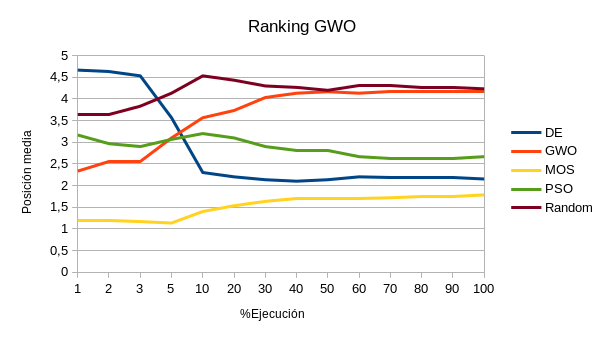
\includegraphics[width=1\textwidth]{Resultados/basico/d10/Grafico_puestos.png} \label{img:ranking-D10}
\end{figure}

Se puede observar que para Dimensión 10, el GWO reporta peores soluciones que otras opciones más conocidas como el PSO y el DE. Como contrincante a batir en el mejor de los casos se impone el algoritmo MOS, que genera las mejores soluciones de los algoritmos elegidos para comparar. Se puede observar que, para este tipo de problemas, en D10, \textit{Diferential evolution} y \textit{Multiple Offpring sample} dan resultados relativamente cercanos entre sí y en la comparativa, por ahora, los mejores. Para análisis de esta dimensión no se hablará de estos dos algoritmos a no ser que se den mejores resultados. El algoritmo a batir para D10 es el \textit{Particle Swarm Optimization (PSO)}.

A tener en cuenta que no siempre da resultados peores que los otros algoritmos. Para la función F04 de la tabla \ref{table:100_ejecD10} se observa como da mejores soluciones que los ''mejores'' algoritmos de la práctica, aunque no es generalizado, para el 100\% de las iteraciones no consigue dar nunca la mejor solución de entre los algoritmos a comparar.




\subsection{D30}

\subsubsection*{1\% Ejecuciones}

\input{Resultados/basico/d30/results_1.tex}
\subsubsection*{50\% Ejecuciones}
\input{Resultados/basico/d30/results_50.tex}

\subsubsection*{100\% Ejecuciones}
\input{Resultados/basico/d30/results_100.tex}

\subsubsection*{Media Puestos}
\input{Resultados/basico/d30/results_mean.tex}
\begin{figure}[H]
    \caption{Ranking GWO vs DE/MOS/PSO Dimensión $\rightarrow$ 30}
    \centering
    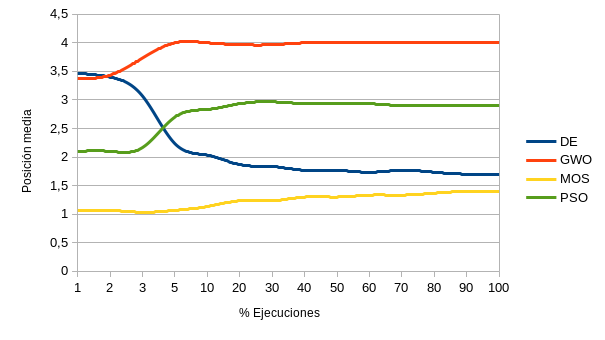
\includegraphics[width=0.8\textwidth]{Resultados/basico/d30/Grafico_puestos.png} \label{img:ranking_D30}
\end{figure}






\section{Hibridación }

Para hibridar el algoritmo de GWO he probado dos versiones. La primera sería una búsqueda local con las características indicadas en el guion de la práctica 1 para el problema del APC. Y la segunda correspondería al algoritmo de Enfriamiento simulado, el cual usa el esquema de enfriamiento de Cauchí modificado explicado en la práctica 3 de la asignatura, se mantienen otras características indicadas en los guiones en los algoritmos implementados.



\subsection{Proceso de Hibridación}

Tanto para el modelo híbrido con enfriamiento simulado como para el de búsqueda local se dan como máximo 200 evaluaciones por ejecución del algoritmo. Estos se ejecutan cada 20 iteraciones sobre los lobos $X_\alpha,X_\beta,X_\delta$ después de calcular los desplazamientos y los nuevos fitnes.

Para decidir que versión comparar con el resto de algoritmos vamos a comparar la versión sin hibridar con las otras dos y compararemos la versión hibrida que mejor resultados dé en comparación con su contrincante.


\subsubsection*{Dimensión 10}

\begin{figure}[H]
    \caption{Comparativa GWO vs GWO+LS vs GWO+SA Dimension 10}
    \centering
    \begin{subfigure}[b]{0.49\textwidth}
        \caption{Ranking de Posiciones medias}
        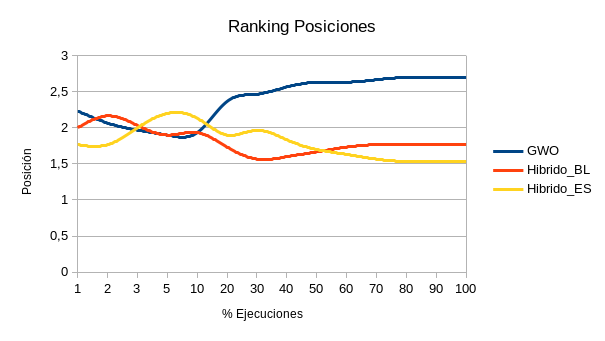
\includegraphics[width=\textwidth]{Resultados/hibrido/Interno/D10/media_posicion.png} \label{img:media_posicion_D10_comparativa}
    \end{subfigure}
    \begin{subfigure}[b]{0.49\textwidth}
        \caption{Error Medio por función al 100\% ejecuciones}
        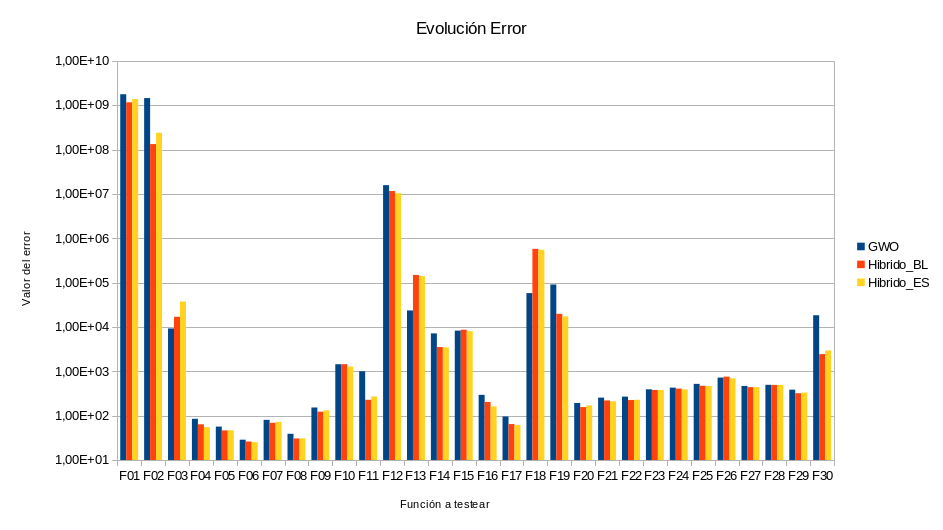
\includegraphics[width=\textwidth]{Resultados/hibrido/Interno/D10/ev_error.png} \label{img:error_D10_comparativa}
    \end{subfigure}

\end{figure}



\input{Resultados/hibrido/Interno/D10/results_mean.tex}




\subsubsection*{Dimensión 30}

\begin{figure}[H]
    \caption{Comparativa GWO vs GWO+LS vs GWO+SA Dimensión 30}
    \centering
    \begin{subfigure}[b]{0.49\textwidth}
        \caption{Ranking de Posiciones medias}

        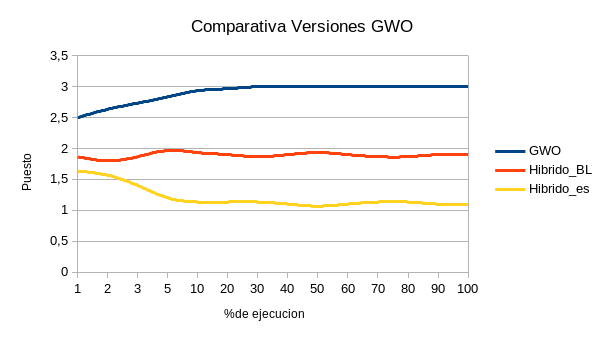
\includegraphics[width=\textwidth]{Resultados/hibrido/Interno/D30/media_posicion.png} \label{img:media_posicion_D30_comparativa}

    \end{subfigure}
    \begin{subfigure}[b]{0.49\textwidth}
        \caption{Error Medio por función al 100\% ejecuciones}
        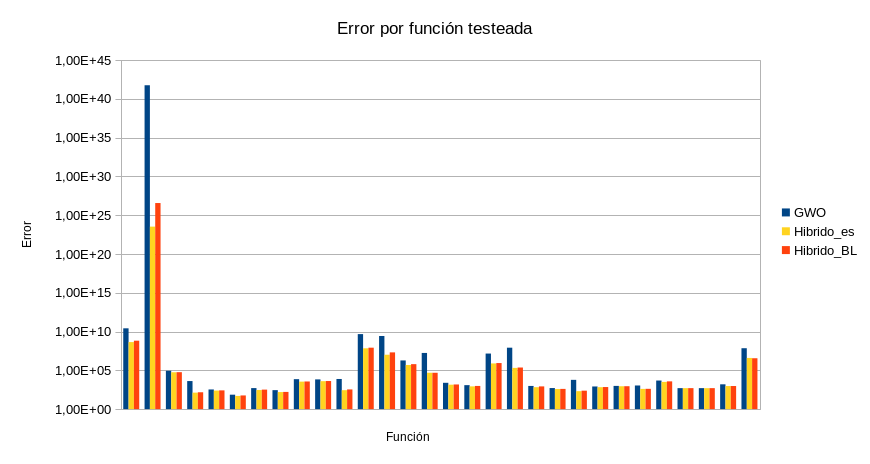
\includegraphics[width=\textwidth]{Resultados/hibrido/Interno/D30/ev_error.png} \label{img:error_D30_comparativa}

    \end{subfigure}

\end{figure}


\input{Resultados/hibrido/Interno/D30/results_mean.tex}



\subsubsection*{Análisis y toma de decisiones}
Ambas versiones proporcionan unos mejores resultados. Siendo la versión de enfriamiento simulado la que gana por poco. Por los resultados de las prácticas tenía cierta noción de qué enfriamiento simulado funciona mejor. Ahora con estos resultados, y después de probarlos en dos tipos de problemas, puedo confirmarlo. La probabilidad de aceptar peores soluciones hace que se estanque en menos mínimos locales y acabe acercándose más a los mínimos globales. También queda claro que, aunque el algoritmo base del GWO tiene mecanismos para explotar el entorno, siempre viene bien utilizar metaheurísticas pensadas para ese objetivo, ya que tenderán a mejorar más los resultados.

Parte de la mejora potencial puede venir de la actualización en la versión híbrida de los lobos $X_\alpha,X_\beta,X_\delta$, que sufren una actualización de sus valores por la ejecución del algoritmo de explotación sobre la solución que almacenaban estos lobos. En la versión original, los lobos $X_\alpha,X_\beta,X_\delta$ no se actualizan a no ser que pierdan su status y pasen a ser $X_\omega$s.

Para el análisis con el resto de algoritmos usaré a partir de ahora el algoritmo hibridado con la búsqueda local. Esta será la versión que se ejecute por defecto en el ejecutable cuando se escoja la versión hibridada. Para más información al respecto, acuda a la sección \ref{subsec:set-up}



\section{Mejoras teóricas}
Al ser una metaheurística poblacional, además basada en comportamientos animales, podemos incluir nuevos operadores que muten los agentes de exploración. Por ejemplo, se podría implementar la reproducción como un sistema elitista en la que la peor solución de la población se reemplaza por una combinación de las mejores soluciones ($X_\alpha$/$X_\beta$/$X_\delta$). Esta mejora en concreto se ha implementado en una versión propia dentro de los ejecutables.



\subsection{Pseudocódigo de la mejora}

A nivel del código del algoritmo básico se mantendría básicamente con la misma estructura:

\begin{algorithm}[H]
    \caption{Grey Wolf Optimization Elitista}\label{alg:GWO_mejorado}
    \begin{algorithmic}[1]
        \Function{GWOE}{$n\_sol,fitnes\_func,min,max,max\_evals$}
        \State Inicializamos la población $X_i (i=1,...,N\_SOL)$
        \State for\_each(agente) $ \gets fitnes\_func(agente)$
        \State $X_\alpha \gets$ Mejor Sol de la población
        \State $X_\beta \gets$ Segunda mejor Sol de la población
        \State $X_\delta \gets$ Tercera mejor Sol de la población
        \State $Max\_iters=max\_evals/N_SOL$
        \For{iter $\in$ Max\_Iters}
        \State $a=2*(1-(iter/max\_evals))$
        \State actualiza\_lobos (dim, población, $\alpha$, $\beta$, $\delta$, a)
        \State for\_each(agente) $ \gets fitnes\_func(agente)$

        \State $X_\alpha \gets$ Mejor Sol de la población
        \State $X_\beta \gets$ Segunda mejor Sol de la población
        \State $X_\delta \gets$ Tercera mejor Sol de la población

        \State $poblacion \gets reproduce(poblacion)$ \Comment{Aplica un operador de cruce a los lobos top de la jerarquía, desplazando con los nuevos lobos a las peores soluciones.}


        \EndFor

        \Return $X_\alpha $
        \EndFunction


    \end{algorithmic}
\end{algorithm}


El algoritmo reproduce se encarga de generar 4 hijos, 2 de la pareja de lobos (soluciones) $X_\alpha$ y $X_\beta$ y 2 de la pareja de lobos (soluciones) $X_\alpha$ y $X_\delta$. Aplicando para la generación de los hijos el algoritmo de cruce BLX explicado en la práctica número 2 de la asignatura debido a que este operador de cruce fue el que mejores resultados dio a la persona que me explicó como implementar el algoritmo de cruce (yo realicé el problema del QAP para las prácticas y el operador de cruce lo he pedido prestado).

El pseudocódigo del algoritmo de reproducción sería:
\begin{algorithm}[H]
    \caption{Algoritmo encargado de la reproducción de la población}
    \begin{algorithmic}[1]
        \Function{reproduccion}{$fitnes, poblacion, alpha, beta, delta, min, max$}
        \State $l1, l2, \gets$ \Call{BLX}{$alpha, beta, min, max$}
        \State $l3, l4, \gets$ \Call{BLX}{$alpha, delta, min, max$}

        \State $l1.fitness \gets fitnes(\&l1.sol[0])$
        \State $l2.fitness \gets fitnes(\&l2.sol[0])$
        \State $l3.fitness \gets fitnes(\&l3.sol[0])$
        \State $l4.fitness \gets fitnes(\&l4.sol[0])$
        \State $tam \gets$ Tamaño de $poblacion$
        \State $poblacion[tam - 1] \gets l1$
        \State $poblacion[tam - 2] \gets l2$
        \State $poblacion[tam - 3] \gets l3$
        \State $poblacion[tam - 4] \gets l4$
        \State Ordenar $poblacion$ por orden ascendente de fitness
        \EndFunction
    \end{algorithmic}


\end{algorithm}

\begin{algorithm}[H]
    \caption{Operador de Cruce BLX}
    \begin{algorithmic}[1]
        \Function{BLX}{$padre1, padre2, min, max$}
        \State $hijo1 \gets padre1->sol$
        \State $hijo2 \gets padre2->sol$
        \State $coef\_max \gets \Call{vmax}{padre1.get()->sol, padre2.get()->sol}$ \Comment{Mayores valores elemento a elemento de la solución}
        \State $coef\_min \gets \Call{vmin}{padre1.get()->sol, padre2.get()->sol}$\Comment{Menores valores elemento a elemento de la solución}
        \State $diff, interv\_x, interv\_y \gets 0$
        \For{$i \gets 0$ to tamaño de $coef\_max$}
        \State $diff \gets coef\_max[i] - coef\_min[i]$
        \State $interv\_x \gets coef\_min[i] - diff * ALFA\_BLX$
        \State $interv\_y \gets coef\_max[i] + diff * ALFA\_BLX$
        \State $hijo1->sol[i] \gets truncar(Random::get(interv\_x, interv\_y), min, max)$
        \State $hijo2->sol[i] \gets truncar(Random::get(interv\_x, interv\_y), min, max)$

        \EndFor
        \State \Return $\{\Call{std::move}{hijo1}, \Call{std::move}{hijo2}\}$
        \EndFunction
    \end{algorithmic}


\end{algorithm}


\subsection{Otras mejoras teóricas}

Otra posible mejora sería la inclusión de nuevos estratos sociales que aportan de manera ponderada al desplazamiento (esto supondría un aumento en el número de agentes que conforman la población). Podría ser por ejemplo 1 alpha, dos beta y tres gamma, cada uno genera un desplazammiento para los omegas, el desplazamiento total será la media de los 3 desplazamientos medios de los lobos con mejores soluciones.

Otra posible mejora sería el control del parametro ''a'' que en el algoritmo básico va de 2 a 0 de manera lineal pero podría tener otros comportamientos (evolución logaritmica u similar). Con este enfoque he encontrado esta implementación en github que propone 2 maneras distintas de calcular ''a'' a parte de la propuesta por el creador de la metaheurística. \url{https://github.com/czeslavo/gwo/tree/master}



\section{Análisis del rendimiento con Mejoras}

En este apartado compararemos la versión básica del algoritmo, la versión con el operador de reproducción extra y una hibridación de la versión básica del algoritmo. Se compararán con los algoritmos ya usados anteriormente para comparar. EL \textit{PSO},\textit{DE} y \textit{MOS}. Primero se comparan las distintas versiones del algoritmo entre sí y luego se compararán con los algoritmos anteriormente indicados.

\subsection{D10}

\subsubsection{Comparativa interna}


\input{Resultados/Analisis_final/D10/GWO/results_100.tex}

\input{Resultados/Analisis_final/D10/GWO/results_mean.tex}


\begin{figure}[H]
    \centering
    \caption{Ranking posiciones medias GWO, GWO+SA y GWO (Mejora elitismo). Dimensión 10}
    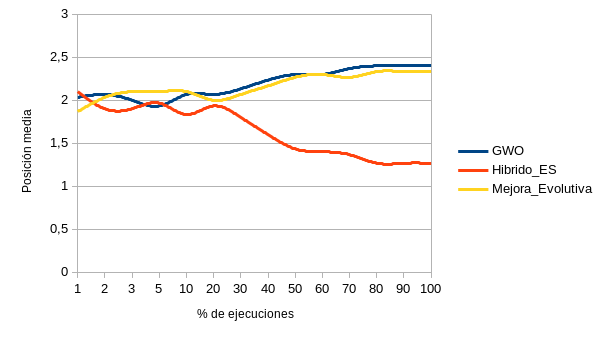
\includegraphics[width=0.9\textwidth]{Resultados/Analisis_final/D10/GWO/Grafico_puestos.png}

\end{figure}

La versión con mejoras teóricas (aplicación de operador de cruce) mejora los resultados, pero no de una manera pronunciada, podría deberse a que, al generarse solo 4 hijos de los mejores lobos y ser la población mucho mayor (50) no tenga un efecto muy medible en el algoritmo.

Por otro lado, al hibridarlo sí que se consigue una mejora sustancial en la diferencia de resultados. Aunque el algoritmo de ES solo se aplica a los lobos líderes (en este caso 3), al ser estos los que dirigen la búsqueda, se consigue escapar de mínimos locales y acaban mejorando el rendimiento general del algoritmo con un pequeño incremento en los tiempos de ejecución




\subsubsection{Comparativa externa}

\input{Resultados/Analisis_final/D10/Todos/results_100.tex}

\input{Resultados/Analisis_final/D10/Todos/results_mean.tex}


\begin{figure}[H]
    \centering
    \caption{Ranking posiciones medias GWO, GWO+SA y GWO(Mejora elitismo) vs PSO,DE y MOS. Dimensión 10}
    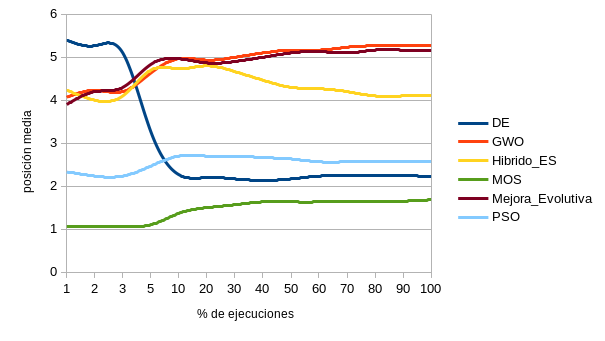
\includegraphics[width=0.9\textwidth]{Resultados/Analisis_final/D10/Todos/Grafico_puestos.png}

\end{figure}


En el gráfico del ranking se puede observar que, en general, este algoritmo y sus modificaciones no son mejores que otras técnicas para la resolución de los problemas del benchmark CEC2017.

\subsection{D30}


\subsubsection{Comparativa interna}


\input{Resultados/Analisis_final/D30/GWO/results_100.tex}

\input{Resultados/Analisis_final/D30/GWO/results_mean.tex}


\begin{figure}[H]
    \centering
    \caption{Ranking posiciones medias GWO, GWO+SA y GWO (Mejora elitismo). Dimensión 10}
    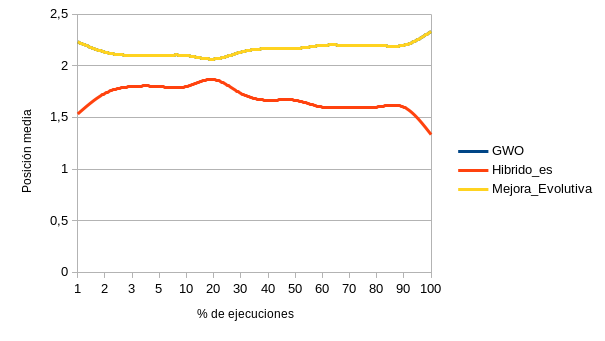
\includegraphics[width=0.9\textwidth]{Resultados/Analisis_final/D30/GWO/Grafico_puestos.png}
    \label{img:aaaaaaaaaaaaaaaaaaaaaaa}

\end{figure}


En estas ejecuciones la versión con la mejora teórica no aporta ninguna mejora, solo un incremento en los tiempos de ejecución que la verdad no dan pié a usar esta versión en dimensiones superiores. Sigue estando presente el razonamiento del apartado anterior, sobre la cantidad de elementos de la población y a cuantos afecta el elitismo. Esto se puede observar en la imagen \ref{img:aaaaaaaaaaaaaaaaaaaaaaa} la cual, a pesar de estar dibujados la evolución de los 3 algoritmos, EL GWO y su versión híbrida dan siempre los mismos resultados


\subsubsection{Comparativa externa}

Tras los resultados del apartado anterior, la comparativa final será ver como responde la versión hibridada del GWO+SA contra el resto de algoritmos antes mencionados.

\input{Resultados/Analisis_final/D30/Todos/results_100.tex}

\input{Resultados/Analisis_final/D30/Todos/results_mean.tex}


\begin{figure}[H]
    \centering
    \caption{Ranking posiciones medias GWO, GWO+SA y GWO(Mejora elitismo) vs PSO,DE y MOS. Dimensión 30}
    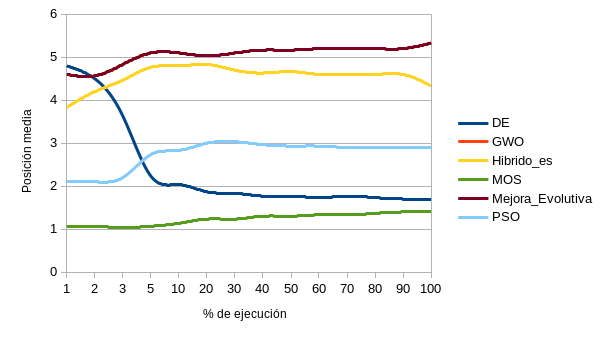
\includegraphics[width=0.9\textwidth]{Resultados/Analisis_final/D30/Todos/Grafico_puestos.png}

\end{figure}

Con la propuesta de hibridación tampoco se mejora ningun algoritmo anteriormente descrito. hasta cierto punto la metaheurística del GWO no rinde a un nivel de competición en los problemas de la compatición CEC2017. Con algunas mejoras en la implementación intuyo que se podrían mejorar algo los resultados aunque no creo que nunca llegen a ser mejores que el algoritmo de \textit{DE}.



\section{Aplicación al problema de las prácticas}

Para la realización de las prácticas escogí el problema del QAP. Como se explica en el siguiente paper: \url{https://ieeexplore.ieee.org/stamp/stamp.jsp?tp=&arnumber=8355479} esta mh no está pensada para la resolución de ese tipo de problemas. Lo que se puede hacer es adaptarla para que se asemeje en comportamiento a la idea original. Por ejemplo, se propone que la nueva solución en vez de ser una media de los 3 desplazamientos, se elija un padre al azar entre los agentes que mejor fitnes tengan. Para el propio operador de cruce se puede implementar una versión del ya existente operador PMX (Partial Mapped Crosover) en el que en vez de elegir dos valores aleatorios para hacer la mezcla, se escoja un rango de la solución aleatorio de tamaño cada vez mayor (Pasar de explorar a explotar como se tenía pensado)


\section{Procedimientos}

Para el desarrollo de la práctica se ha usado el lenguaje de programación C++. Los motivos de esta decisión son: la familiaridad con el lenguaje de programación y el rendimiento superior a lenguajes de programación de alto nivel, conveniente para el tratamiento de grandes cantidades de datos, o la resolución de problemas computacionalmente intensivos.

Para la compilación del código se ha usado el compilador clang (aunque puede usar cualquiera). La estructura del proyecto se ha configurado usando CMAKE. Para la ejecución de los programas se ha usado el sistema operativo Linux. Aunque al usar CMAKE se podría generar un proyecto para Windows.

\subsection{Estructura del proyecto}

El proyecto se ha estructurado de la siguiente manera:


\dirtree{%
    .1 code.
    .2 SRC \DTcomment{Carpeta con el código fuente del proyecto}.
    .2 INCLUDE \DTcomment{Carpeta con los archivos de cabecera del proyecto}.
    .2 Input\_data \DTcomment{Carpeta con los datos para ejecutar los algoritmos}.
    .2 CMakeList.text \DTcomment{Archivo de configuración CMAKE}.
    .2 build \DTcomment{Carpeta donde se recomienda generar los archivos de compilación de CMAKE en caso de compilar}.
    .2 extract\_all.py \DTcomment{Archivo de ejecución de extract.py}.
    .2 extract.py \DTcomment{Genera una hoja de calculo con los archivos de resultado}.
    .2 genera\_medias.py \DTcomment{Genera la media de las distintas ejecuciones en una hoja de calculo para su posterior analisis}.
    .2 Modifica\_tablas.py \DTcomment{Modifica las tablas en latex de \url{tacolab.org} para que estén bien formateadas(necesitan arreglo todavia)}.
    .2 Memoria.pdf.
}


\subsection{Set Up} \label{subsec:set-up}

Se le entregará un archivo .zip llamado software que contendrá la estructura de directorios anterior. La carpeta build estará vacía por cuestiones obvias. Los ejecutables para la plataforma LINUX$\times$64 se encontrarán en la raíz del proyecto.

Si su plataforma no está entre las pre-compiladas, siga leyendo este apartado, sino, salte al apartado de ejecución.

Si no puede ejecutar ninguno de los ejecutables. Deberá tener un compilador de c++ instalado en su computador y el programa \textbf{\textit{CMAKE}} y \textbf{\textit{make}}  para seguir con el tutorial.


\subsubsection*{Linux}

\begin{enumerate}
    \item Abra una terminal en la raíz del proyecto
    \item Si no está creada la carpeta build (que no debería), créela, sino pase al paso 3
          \begin{itemize}
              \item \begin{lstlisting}[language=bash]
				mkdir build
            \end{lstlisting}
          \end{itemize}
    \item Acceda a la carpeta build e inicialice el proyecto
          \begin{itemize}
              \item \begin{lstlisting}[language=bash]
				cd build
				cmake ..
				cd ..
				cmake -DCMAKE_BUILD_TYPE=Release -S . -B build
            \end{lstlisting}
          \end{itemize}
    \item Compile el programa
          \begin{itemize}
              \item \begin{lstlisting}[language=bash]
				cmake --build build --target gwo
            \end{lstlisting}
          \end{itemize}
\end{enumerate}

\subsubsection{Windows}

El programa se ha escrito pensando en ejecutarse en Linux, si se tiene un sistema Windows lo que se recomienda es usar WSL, instalar el compilador de c++ GNU y CMAKE en esa máquina virtual y ejecutar desde ahí, siguiendo las instrucciones del apartado anterior.

\subsection{Ejecución}

Para la ejecución del programa se ha pensado en pasar los parámetros siempre por línea de comandos. El programa permite configurar que ejecutar y como de la siguiente manera:

\begin{figure}[H]
    \centering
    \caption{Flags permitidos por el ejecutable}
    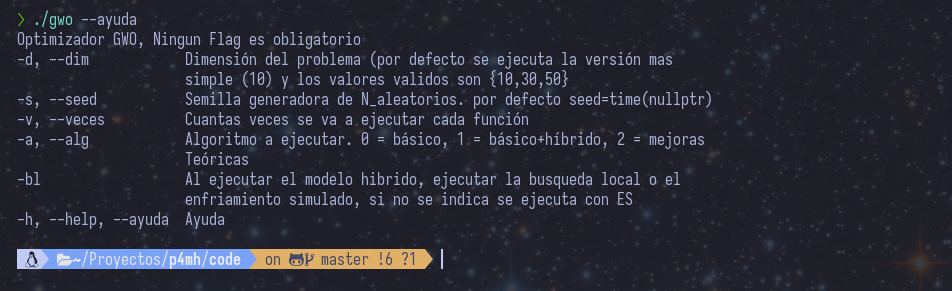
\includegraphics[width=\textwidth]{dash_help_program.png}


\end{figure}

Si el programa se ejecuta sin ningún flag, se ejecutará la versión básica del algoritmo 10 veces con semilla igual a la hora de la cpu en el momento de la ejecución.


\bibliographystyle{alpha}
\bibliography{mybib}


\end{document}
